\documentclass[1p]{elsarticle_modified}
%\bibliographystyle{elsarticle-num}

%\usepackage[colorlinks]{hyperref}
%\usepackage{abbrmath_seonhwa} %\Abb, \Ascr, \Acal ,\Abf, \Afrak
\usepackage{amsfonts}
\usepackage{amssymb}
\usepackage{amsmath}
\usepackage{amsthm}
\usepackage{scalefnt}
\usepackage{amsbsy}
\usepackage{kotex}
\usepackage{caption}
\usepackage{subfig}
\usepackage{color}
\usepackage{graphicx}
\usepackage{xcolor} %% white, black, red, green, blue, cyan, magenta, yellow
\usepackage{float}
\usepackage{setspace}
\usepackage{hyperref}

\usepackage{tikz}
\usetikzlibrary{arrows}

\usepackage{multirow}
\usepackage{array} % fixed length table
\usepackage{hhline}

%%%%%%%%%%%%%%%%%%%%%
\makeatletter
\renewcommand*\env@matrix[1][\arraystretch]{%
	\edef\arraystretch{#1}%
	\hskip -\arraycolsep
	\let\@ifnextchar\new@ifnextchar
	\array{*\c@MaxMatrixCols c}}
\makeatother %https://tex.stackexchange.com/questions/14071/how-can-i-increase-the-line-spacing-in-a-matrix
%%%%%%%%%%%%%%%

\usepackage[normalem]{ulem}

\newcommand{\msout}[1]{\ifmmode\text{\sout{\ensuremath{#1}}}\else\sout{#1}\fi}
%SOURCE: \msout is \stkout macro in https://tex.stackexchange.com/questions/20609/strikeout-in-math-mode

\newcommand{\cancel}[1]{
	\ifmmode
	{\color{red}\msout{#1}}
	\else
	{\color{red}\sout{#1}}
	\fi
}

\newcommand{\add}[1]{
	{\color{blue}\uwave{#1}}
}

\newcommand{\replace}[2]{
	\ifmmode
	{\color{red}\msout{#1}}{\color{blue}\uwave{#2}}
	\else
	{\color{red}\sout{#1}}{\color{blue}\uwave{#2}}
	\fi
}

\newcommand{\Sol}{\mathcal{S}} %segment
\newcommand{\D}{D} %diagram
\newcommand{\A}{\mathcal{A}} %arc


%%%%%%%%%%%%%%%%%%%%%%%%%%%%%5 test

\def\sl{\operatorname{\textup{SL}}(2,\Cbb)}
\def\psl{\operatorname{\textup{PSL}}(2,\Cbb)}
\def\quan{\mkern 1mu \triangleright \mkern 1mu}

\theoremstyle{definition}
\newtheorem{thm}{Theorem}[section]
\newtheorem{prop}[thm]{Proposition}
\newtheorem{lem}[thm]{Lemma}
\newtheorem{ques}[thm]{Question}
\newtheorem{cor}[thm]{Corollary}
\newtheorem{defn}[thm]{Definition}
\newtheorem{exam}[thm]{Example}
\newtheorem{rmk}[thm]{Remark}
\newtheorem{alg}[thm]{Algorithm}

\newcommand{\I}{\sqrt{-1}}
\begin{document}

%\begin{frontmatter}
%
%\title{Boundary parabolic representations of knots up to 8 crossings}
%
%%% Group authors per affiliation:
%\author{Yunhi Cho} 
%\address{Department of Mathematics, University of Seoul, Seoul, Korea}
%\ead{yhcho@uos.ac.kr}
%
%
%\author{Seonhwa Kim} %\fnref{s_kim}}
%\address{Center for Geometry and Physics, Institute for Basic Science, Pohang, 37673, Korea}
%\ead{ryeona17@ibs.re.kr}
%
%\author{Hyuk Kim}
%\address{Department of Mathematical Sciences, Seoul National University, Seoul 08826, Korea}
%\ead{hyukkim@snu.ac.kr}
%
%\author{Seokbeom Yoon}
%\address{Department of Mathematical Sciences, Seoul National University, Seoul, 08826,  Korea}
%\ead{sbyoon15@snu.ac.kr}
%
%\begin{abstract}
%We find all boundary parabolic representation of knots up to 8 crossings.
%
%\end{abstract}
%\begin{keyword}
%    \MSC[2010] 57M25 
%\end{keyword}
%
%\end{frontmatter}

%\linenumbers
%\tableofcontents
%
\newcommand\colored[1]{\textcolor{white}{\rule[-0.35ex]{0.8em}{1.4ex}}\kern-0.8em\color{red} #1}%
%\newcommand\colored[1]{\textcolor{white}{ #1}\kern-2.17ex	\textcolor{white}{ #1}\kern-1.81ex	\textcolor{white}{ #1}\kern-2.15ex\color{red}#1	}

{\Large $\underline{11a_{361}~(K11a_{361})}$}

\setlength{\tabcolsep}{10pt}
\renewcommand{\arraystretch}{1.6}
\vspace{1cm}\begin{tabular}{m{100pt}>{\centering\arraybackslash}m{274pt}}
\multirow{5}{120pt}{
	\centering
	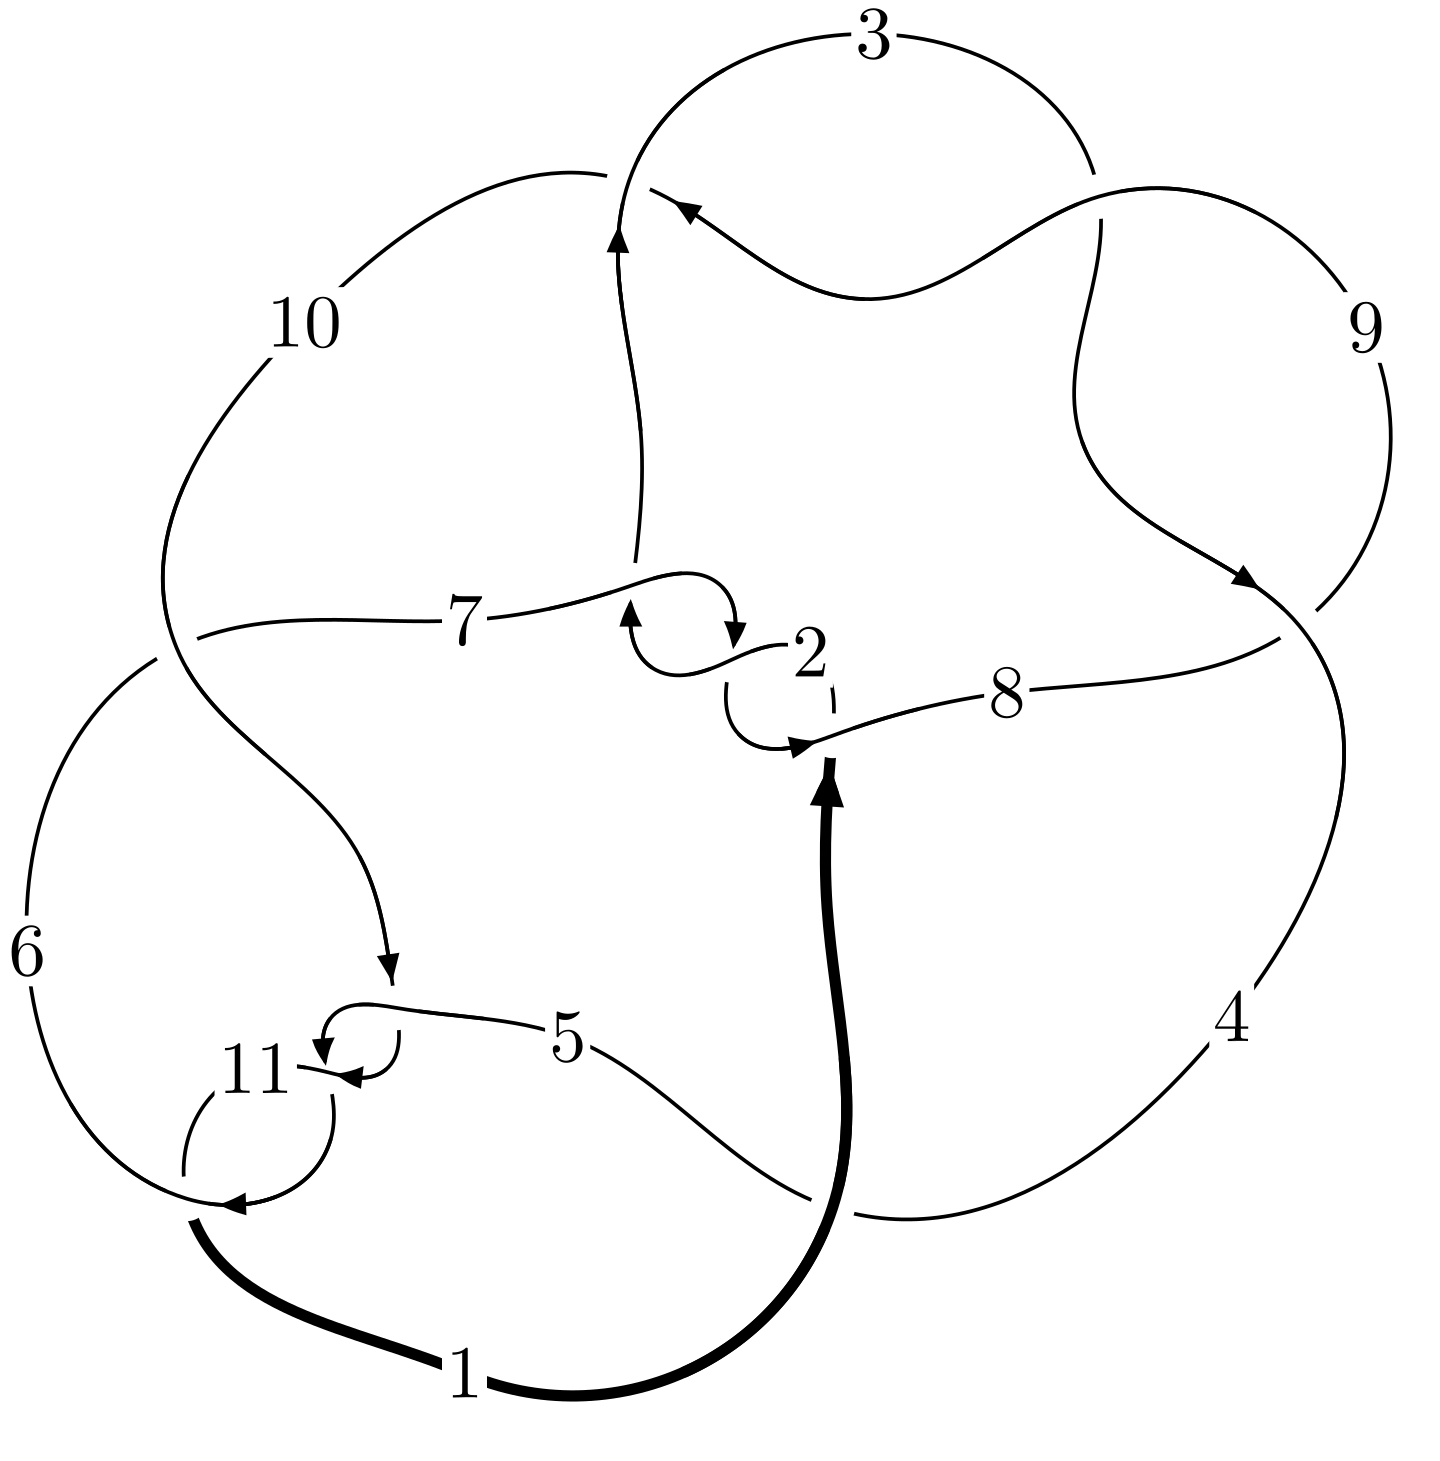
\includegraphics[width=112pt]{../../../GIT/diagram.site/Diagrams/png/610_11a_361.png}\\
\ \ \ A knot diagram\footnotemark}&
\allowdisplaybreaks
\textbf{Linearized knot diagam} \\
\cline{2-2}
 &
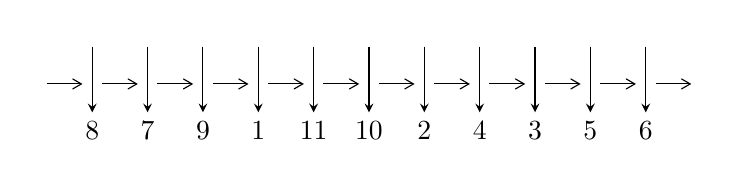
\begin{tikzpicture}[x=20pt, y=17pt]
	% nodes
	\node (C0) at (0, 0) {};
	\node (C1) at (1, 0) {};
	\node (C1U) at (1, +1) {};
	\node (C1D) at (1, -1) {8};

	\node (C2) at (2, 0) {};
	\node (C2U) at (2, +1) {};
	\node (C2D) at (2, -1) {7};

	\node (C3) at (3, 0) {};
	\node (C3U) at (3, +1) {};
	\node (C3D) at (3, -1) {9};

	\node (C4) at (4, 0) {};
	\node (C4U) at (4, +1) {};
	\node (C4D) at (4, -1) {1};

	\node (C5) at (5, 0) {};
	\node (C5U) at (5, +1) {};
	\node (C5D) at (5, -1) {11};

	\node (C6) at (6, 0) {};
	\node (C6U) at (6, +1) {};
	\node (C6D) at (6, -1) {10};

	\node (C7) at (7, 0) {};
	\node (C7U) at (7, +1) {};
	\node (C7D) at (7, -1) {2};

	\node (C8) at (8, 0) {};
	\node (C8U) at (8, +1) {};
	\node (C8D) at (8, -1) {4};

	\node (C9) at (9, 0) {};
	\node (C9U) at (9, +1) {};
	\node (C9D) at (9, -1) {3};

	\node (C10) at (10, 0) {};
	\node (C10U) at (10, +1) {};
	\node (C10D) at (10, -1) {5};

	\node (C11) at (11, 0) {};
	\node (C11U) at (11, +1) {};
	\node (C11D) at (11, -1) {6};
	\node (C12) at (12, 0) {};

	% arrows
	\draw[->,>={angle 60}]
	(C0) edge (C1) (C1) edge (C2) (C2) edge (C3) (C3) edge (C4) (C4) edge (C5) (C5) edge (C6) (C6) edge (C7) (C7) edge (C8) (C8) edge (C9) (C9) edge (C10) (C10) edge (C11) (C11) edge (C12) ;	\draw[->,>=stealth]
	(C1U) edge (C1D) (C2U) edge (C2D) (C3U) edge (C3D) (C4U) edge (C4D) (C5U) edge (C5D) (C6U) edge (C6D) (C7U) edge (C7D) (C8U) edge (C8D) (C9U) edge (C9D) (C10U) edge (C10D) (C11U) edge (C11D) ;
	\end{tikzpicture} \\
\hhline{~~} \\& 
\textbf{Solving Sequence} \\ \cline{2-2} 
 &
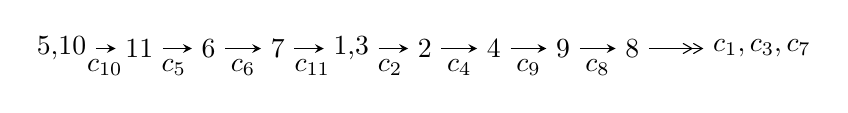
\begin{tikzpicture}[x=25pt, y=7pt]
	% node
	\node (A0) at (-1/8, 0) {5,10};
	\node (A1) at (1, 0) {11};
	\node (A2) at (2, 0) {6};
	\node (A3) at (3, 0) {7};
	\node (A4) at (65/16, 0) {1,3};
	\node (A5) at (41/8, 0) {2};
	\node (A6) at (49/8, 0) {4};
	\node (A7) at (57/8, 0) {9};
	\node (A8) at (65/8, 0) {8};
	\node (C1) at (1/2, -1) {$c_{10}$};
	\node (C2) at (3/2, -1) {$c_{5}$};
	\node (C3) at (5/2, -1) {$c_{6}$};
	\node (C4) at (7/2, -1) {$c_{11}$};
	\node (C5) at (37/8, -1) {$c_{2}$};
	\node (C6) at (45/8, -1) {$c_{4}$};
	\node (C7) at (53/8, -1) {$c_{9}$};
	\node (C8) at (61/8, -1) {$c_{8}$};
	\node (A9) at (10, 0) {$c_{1},c_{3},c_{7}$};

	% edge
	\draw[->,>=stealth]	
	(A0) edge (A1) (A1) edge (A2) (A2) edge (A3) (A3) edge (A4) (A4) edge (A5) (A5) edge (A6) (A6) edge (A7) (A7) edge (A8) ;
	\draw[->>,>={angle 60}]	
	(A8) edge (A9);
\end{tikzpicture} \\ 

\end{tabular} \\

\footnotetext{
The image of knot diagram is generated by the software ``\textbf{Draw programme}" developed by Andrew Bartholomew(\url{http://www.layer8.co.uk/maths/draw/index.htm\#Running-draw}), where we modified some parts for our purpose(\url{https://github.com/CATsTAILs/LinksPainter}).
}\phantom \\ \newline 
\centering \textbf{Ideals for irreducible components\footnotemark of $X_{\text{par}}$} 
 
\begin{align*}
I^u_{1}&=\langle 
- u^{17}+2 u^{16}+\cdots+b-1,\;-5 u^{17}+9 u^{16}+\cdots+2 a-7,\;u^{18}-3 u^{17}+\cdots-7 u-2\rangle \\
I^u_{2}&=\langle 
u^{10} a- u^{10}+\cdots+2 a-1,\;2 u^{10} a- u^{10}+\cdots+a-3,\\
\phantom{I^u_{2}}&\phantom{= \langle  }u^{11}+u^{10}-4 u^9-3 u^8+6 u^7+2 u^6-2 u^5+3 u^4-3 u^3-3 u^2+2 u-1\rangle \\
I^u_{3}&=\langle 
u^5-2 u^3+b+u,\;- u^5+3 u^3- u^2+a-2 u+1,\;u^6-3 u^4+2 u^2+1\rangle \\
\\
\end{align*}
\raggedright * 3 irreducible components of $\dim_{\mathbb{C}}=0$, with total 46 representations.\\
\footnotetext{All coefficients of polynomials are rational numbers. But the coefficients are sometimes approximated in decimal forms when there is not enough margin.}
\newpage
\renewcommand{\arraystretch}{1}
\centering \section*{I. $I^u_{1}= \langle - u^{17}+2 u^{16}+\cdots+b-1,\;-5 u^{17}+9 u^{16}+\cdots+2 a-7,\;u^{18}-3 u^{17}+\cdots-7 u-2 \rangle$}
\flushleft \textbf{(i) Arc colorings}\\
\begin{tabular}{m{7pt} m{180pt} m{7pt} m{180pt} }
\flushright $a_{5}=$&$\begin{pmatrix}0\\u\end{pmatrix}$ \\
\flushright $a_{10}=$&$\begin{pmatrix}1\\0\end{pmatrix}$ \\
\flushright $a_{11}=$&$\begin{pmatrix}1\\u^2\end{pmatrix}$ \\
\flushright $a_{6}=$&$\begin{pmatrix}- u\\- u^3+u\end{pmatrix}$ \\
\flushright $a_{7}=$&$\begin{pmatrix}u^3-2 u\\- u^3+u\end{pmatrix}$ \\
\flushright $a_{1}=$&$\begin{pmatrix}- u^2+1\\- u^4+2 u^2\end{pmatrix}$ \\
\flushright $a_{3}=$&$\begin{pmatrix}\frac{5}{2} u^{17}-\frac{9}{2} u^{16}+\cdots+16 u+\frac{7}{2}\\u^{17}-2 u^{16}+\cdots+6 u+1\end{pmatrix}$ \\
\flushright $a_{2}=$&$\begin{pmatrix}\frac{3}{2} u^{17}-\frac{5}{2} u^{16}+\cdots+9 u+\frac{3}{2}\\u^{17}-2 u^{16}+\cdots+5 u+1\end{pmatrix}$ \\
\flushright $a_{4}=$&$\begin{pmatrix}u^5-2 u^3+u\\u^7-3 u^5+2 u^3+u\end{pmatrix}$ \\
\flushright $a_{9}=$&$\begin{pmatrix}\frac{1}{2} u^{17}-\frac{1}{2} u^{16}+\cdots+3 u+\frac{3}{2}\\- u^{17}+u^{16}+\cdots-4 u-1\end{pmatrix}$ \\
\flushright $a_{8}=$&$\begin{pmatrix}\frac{1}{2} u^{17}-\frac{1}{2} u^{16}+\cdots+4 u+\frac{3}{2}\\-2 u^{17}+3 u^{16}+\cdots-12 u-3\end{pmatrix}$\\ \flushright $a_{8}=$&$\begin{pmatrix}\frac{1}{2} u^{17}-\frac{1}{2} u^{16}+\cdots+4 u+\frac{3}{2}\\-2 u^{17}+3 u^{16}+\cdots-12 u-3\end{pmatrix}$\\&\end{tabular}
\flushleft \textbf{(ii) Obstruction class $= -1$}\\~\\
\flushleft \textbf{(iii) Cusp Shapes $= -4 u^{17}+4 u^{16}+26 u^{15}-16 u^{14}-76 u^{13}+10 u^{12}+112 u^{11}+58 u^{10}-50 u^9-126 u^8-88 u^7+58 u^6+122 u^5+70 u^4-12 u^3-50 u^2-46 u-30$}\\~\\
\newpage\renewcommand{\arraystretch}{1}
\flushleft \textbf{(iv) u-Polynomials at the component}\newline \\
\begin{tabular}{m{50pt}|m{274pt}}
Crossings & \hspace{64pt}u-Polynomials at each crossing \\
\hline $$\begin{aligned}c_{1},c_{2},c_{3}\\c_{7},c_{8},c_{9}\end{aligned}$$&$\begin{aligned}
&u^{18}+12 u^{16}+\cdots-3 u-1
\end{aligned}$\\
\hline $$\begin{aligned}c_{4},c_{6}\end{aligned}$$&$\begin{aligned}
&u^{18}+9 u^{17}+\cdots+223 u+26
\end{aligned}$\\
\hline $$\begin{aligned}c_{5},c_{10},c_{11}\end{aligned}$$&$\begin{aligned}
&u^{18}-3 u^{17}+\cdots-7 u-2
\end{aligned}$\\
\hline
\end{tabular}\\~\\
\newpage\renewcommand{\arraystretch}{1}
\flushleft \textbf{(v) Riley Polynomials at the component}\newline \\
\begin{tabular}{m{50pt}|m{274pt}}
Crossings & \hspace{64pt}Riley Polynomials at each crossing \\
\hline $$\begin{aligned}c_{1},c_{2},c_{3}\\c_{7},c_{8},c_{9}\end{aligned}$$&$\begin{aligned}
&y^{18}+24 y^{17}+\cdots-5 y+1
\end{aligned}$\\
\hline $$\begin{aligned}c_{4},c_{6}\end{aligned}$$&$\begin{aligned}
&y^{18}+13 y^{17}+\cdots-7609 y+676
\end{aligned}$\\
\hline $$\begin{aligned}c_{5},c_{10},c_{11}\end{aligned}$$&$\begin{aligned}
&y^{18}-15 y^{17}+\cdots-41 y+4
\end{aligned}$\\
\hline
\end{tabular}\\~\\
\newpage\flushleft \textbf{(vi) Complex Volumes and Cusp Shapes}
$$\begin{array}{c|c|c}  
\text{Solutions to }I^u_{1}& \I (\text{vol} + \sqrt{-1}CS) & \text{Cusp shape}\\
 \hline 
\begin{aligned}
u &= -0.123856 + 0.896133 I \\
a &= -0.64726 - 2.44716 I \\
b &= -0.30161 + 1.61404 I\end{aligned}
 & \phantom{-}16.3220 + 7.5688 I & -2.56060 - 3.84684 I \\ \hline\begin{aligned}
u &= -0.123856 - 0.896133 I \\
a &= -0.64726 + 2.44716 I \\
b &= -0.30161 - 1.61404 I\end{aligned}
 & \phantom{-}16.3220 - 7.5688 I & -2.56060 + 3.84684 I \\ \hline\begin{aligned}
u &= -0.538460 + 0.620351 I \\
a &= \phantom{-}1.03715 + 1.21621 I \\
b &= \phantom{-}0.05142 - 1.55107 I\end{aligned}
 & \phantom{-}10.10640 + 2.19718 I & -4.14124 - 3.09555 I \\ \hline\begin{aligned}
u &= -0.538460 - 0.620351 I \\
a &= \phantom{-}1.03715 - 1.21621 I \\
b &= \phantom{-}0.05142 + 1.55107 I\end{aligned}
 & \phantom{-}10.10640 - 2.19718 I & -4.14124 + 3.09555 I \\ \hline\begin{aligned}
u &= -1.151600 + 0.470809 I \\
a &= -0.509790 - 1.091590 I \\
b &= \phantom{-}0.24523 + 1.63308 I\end{aligned}
 & \phantom{-}13.17120 - 2.70335 I & -5.20794 + 0.16548 I \\ \hline\begin{aligned}
u &= -1.151600 - 0.470809 I \\
a &= -0.509790 + 1.091590 I \\
b &= \phantom{-}0.24523 - 1.63308 I\end{aligned}
 & \phantom{-}13.17120 + 2.70335 I & -5.20794 - 0.16548 I \\ \hline\begin{aligned}
u &= -1.261310 + 0.252068 I \\
a &= \phantom{-}0.211990 + 0.318908 I \\
b &= -0.236066 - 0.509153 I\end{aligned}
 & -1.47242 + 2.06370 I & -11.90510 + 0.97448 I \\ \hline\begin{aligned}
u &= -1.261310 - 0.252068 I \\
a &= \phantom{-}0.211990 - 0.318908 I \\
b &= -0.236066 + 0.509153 I\end{aligned}
 & -1.47242 - 2.06370 I & -11.90510 - 0.97448 I \\ \hline\begin{aligned}
u &= -0.031986 + 0.701532 I \\
a &= -0.175359 + 1.101380 I \\
b &= \phantom{-}0.386143 - 0.454390 I\end{aligned}
 & \phantom{-}2.29851 + 1.35610 I & -7.33537 - 5.27531 I \\ \hline\begin{aligned}
u &= -0.031986 - 0.701532 I \\
a &= -0.175359 - 1.101380 I \\
b &= \phantom{-}0.386143 + 0.454390 I\end{aligned}
 & \phantom{-}2.29851 - 1.35610 I & -7.33537 + 5.27531 I\\
 \hline 
 \end{array}$$\newpage$$\begin{array}{c|c|c}  
\text{Solutions to }I^u_{1}& \I (\text{vol} + \sqrt{-1}CS) & \text{Cusp shape}\\
 \hline 
\begin{aligned}
u &= \phantom{-}1.30632\phantom{ +0.000000I} \\
a &= \phantom{-}0.919432\phantom{ +0.000000I} \\
b &= \phantom{-}0.613328\phantom{ +0.000000I}\end{aligned}
 & -5.28445\phantom{ +0.000000I} & -18.9030\phantom{ +0.000000I} \\ \hline\begin{aligned}
u &= \phantom{-}1.286650 + 0.297323 I \\
a &= -0.675519 + 0.845692 I \\
b &= -0.521429 - 0.448538 I\end{aligned}
 & -1.81273 - 4.98441 I & -12.9081 + 7.6610 I \\ \hline\begin{aligned}
u &= \phantom{-}1.286650 - 0.297323 I \\
a &= -0.675519 - 0.845692 I \\
b &= -0.521429 + 0.448538 I\end{aligned}
 & -1.81273 + 4.98441 I & -12.9081 - 7.6610 I \\ \hline\begin{aligned}
u &= \phantom{-}1.36136 + 0.40071 I \\
a &= \phantom{-}1.71836 - 1.08684 I \\
b &= \phantom{-}0.33798 + 1.58437 I\end{aligned}
 & \phantom{-}11.6528 - 12.2200 I & -6.45692 + 6.09309 I \\ \hline\begin{aligned}
u &= \phantom{-}1.36136 - 0.40071 I \\
a &= \phantom{-}1.71836 + 1.08684 I \\
b &= \phantom{-}0.33798 - 1.58437 I\end{aligned}
 & \phantom{-}11.6528 + 12.2200 I & -6.45692 - 6.09309 I \\ \hline\begin{aligned}
u &= \phantom{-}1.45252 + 0.15463 I \\
a &= -0.916883 - 0.366782 I \\
b &= -0.11443 - 1.46229 I\end{aligned}
 & \phantom{-}3.61426 - 4.76803 I & -7.92624 + 3.38619 I \\ \hline\begin{aligned}
u &= \phantom{-}1.45252 - 0.15463 I \\
a &= -0.916883 + 0.366782 I \\
b &= -0.11443 + 1.46229 I\end{aligned}
 & \phantom{-}3.61426 + 4.76803 I & -7.92624 - 3.38619 I \\ \hline\begin{aligned}
u &= -0.292956\phantom{ +0.000000I} \\
a &= -0.504799\phantom{ +0.000000I} \\
b &= -0.307793\phantom{ +0.000000I}\end{aligned}
 & -0.489564\phantom{ +0.000000I} & -20.2140\phantom{ +0.000000I}\\
 \hline 
 \end{array}$$\newpage\newpage\renewcommand{\arraystretch}{1}
\centering \section*{II. $I^u_{2}= \langle u^{10} a- u^{10}+\cdots+2 a-1,\;2 u^{10} a- u^{10}+\cdots+a-3,\;u^{11}+u^{10}+\cdots+2 u-1 \rangle$}
\flushleft \textbf{(i) Arc colorings}\\
\begin{tabular}{m{7pt} m{180pt} m{7pt} m{180pt} }
\flushright $a_{5}=$&$\begin{pmatrix}0\\u\end{pmatrix}$ \\
\flushright $a_{10}=$&$\begin{pmatrix}1\\0\end{pmatrix}$ \\
\flushright $a_{11}=$&$\begin{pmatrix}1\\u^2\end{pmatrix}$ \\
\flushright $a_{6}=$&$\begin{pmatrix}- u\\- u^3+u\end{pmatrix}$ \\
\flushright $a_{7}=$&$\begin{pmatrix}u^3-2 u\\- u^3+u\end{pmatrix}$ \\
\flushright $a_{1}=$&$\begin{pmatrix}- u^2+1\\- u^4+2 u^2\end{pmatrix}$ \\
\flushright $a_{3}=$&$\begin{pmatrix}a\\-\frac{1}{3} u^{10} a+\frac{1}{3} u^{10}+\cdots-\frac{2}{3} a+\frac{1}{3}\end{pmatrix}$ \\
\flushright $a_{2}=$&$\begin{pmatrix}-\frac{1}{3} u^{10} a-\frac{2}{3} u^{10}+\cdots+\frac{1}{3} a-\frac{2}{3}\\-\frac{1}{3} u^{10} a+u^{10}+\cdots-\frac{1}{3} a+\frac{1}{3}\end{pmatrix}$ \\
\flushright $a_{4}=$&$\begin{pmatrix}u^5-2 u^3+u\\u^7-3 u^5+2 u^3+u\end{pmatrix}$ \\
\flushright $a_{9}=$&$\begin{pmatrix}-\frac{2}{3} u^{10} a-\frac{2}{3} u^9 a+\cdots+\frac{1}{3} a+\frac{5}{3}\\-\frac{1}{3} u^{10} a-\frac{1}{3} u^{10}+\cdots+\frac{1}{3} u+\frac{1}{3}\end{pmatrix}$ \\
\flushright $a_{8}=$&$\begin{pmatrix}-\frac{1}{3} u^{10} a+\frac{1}{3} u^{10}+\cdots+\frac{1}{3} a+\frac{4}{3}\\\frac{1}{3} u^{10} a+\frac{1}{3} u^9 a+\cdots+\frac{1}{3} a+\frac{2}{3}\end{pmatrix}$\\ \flushright $a_{8}=$&$\begin{pmatrix}-\frac{1}{3} u^{10} a+\frac{1}{3} u^{10}+\cdots+\frac{1}{3} a+\frac{4}{3}\\\frac{1}{3} u^{10} a+\frac{1}{3} u^9 a+\cdots+\frac{1}{3} a+\frac{2}{3}\end{pmatrix}$\\&\end{tabular}
\flushleft \textbf{(ii) Obstruction class $= -1$}\\~\\
\flushleft \textbf{(iii) Cusp Shapes $= -4 u^9+16 u^7-4 u^6-20 u^5+12 u^4-4 u^3-8 u^2+20 u-14$}\\~\\
\newpage\renewcommand{\arraystretch}{1}
\flushleft \textbf{(iv) u-Polynomials at the component}\newline \\
\begin{tabular}{m{50pt}|m{274pt}}
Crossings & \hspace{64pt}u-Polynomials at each crossing \\
\hline $$\begin{aligned}c_{1},c_{2},c_{3}\\c_{7},c_{8},c_{9}\end{aligned}$$&$\begin{aligned}
&u^{22}- u^{21}+\cdots+6 u+5
\end{aligned}$\\
\hline $$\begin{aligned}c_{4},c_{6}\end{aligned}$$&$\begin{aligned}
&(u^{11}-3 u^{10}+\cdots-2 u+1)^{2}
\end{aligned}$\\
\hline $$\begin{aligned}c_{5},c_{10},c_{11}\end{aligned}$$&$\begin{aligned}
&(u^{11}+u^{10}-4 u^9-3 u^8+6 u^7+2 u^6-2 u^5+3 u^4-3 u^3-3 u^2+2 u-1)^2
\end{aligned}$\\
\hline
\end{tabular}\\~\\
\newpage\renewcommand{\arraystretch}{1}
\flushleft \textbf{(v) Riley Polynomials at the component}\newline \\
\begin{tabular}{m{50pt}|m{274pt}}
Crossings & \hspace{64pt}Riley Polynomials at each crossing \\
\hline $$\begin{aligned}c_{1},c_{2},c_{3}\\c_{7},c_{8},c_{9}\end{aligned}$$&$\begin{aligned}
&y^{22}+19 y^{21}+\cdots+24 y+25
\end{aligned}$\\
\hline $$\begin{aligned}c_{4},c_{6}\end{aligned}$$&$\begin{aligned}
&(y^{11}+11 y^{10}+\cdots+6 y-1)^{2}
\end{aligned}$\\
\hline $$\begin{aligned}c_{5},c_{10},c_{11}\end{aligned}$$&$\begin{aligned}
&(y^{11}-9 y^{10}+\cdots-2 y-1)^{2}
\end{aligned}$\\
\hline
\end{tabular}\\~\\
\newpage\flushleft \textbf{(vi) Complex Volumes and Cusp Shapes}
$$\begin{array}{c|c|c}  
\text{Solutions to }I^u_{2}& \I (\text{vol} + \sqrt{-1}CS) & \text{Cusp shape}\\
 \hline 
\begin{aligned}
u &= \phantom{-}1.14725\phantom{ +0.000000I} \\
a &= -1.48144 + 0.67002 I \\
b &= -0.301144 - 1.127860 I\end{aligned}
 & \phantom{-}1.09450\phantom{ +0.000000I} & -7.62370\phantom{ +0.000000I} \\ \hline\begin{aligned}
u &= \phantom{-}1.14725\phantom{ +0.000000I} \\
a &= -1.48144 - 0.67002 I \\
b &= -0.301144 + 1.127860 I\end{aligned}
 & \phantom{-}1.09450\phantom{ +0.000000I} & -7.62370\phantom{ +0.000000I} \\ \hline\begin{aligned}
u &= \phantom{-}0.044199 + 0.849205 I \\
a &= \phantom{-}0.388928 + 0.983366 I \\
b &= -0.915282 - 0.626510 I\end{aligned}
 & \phantom{-}8.93247 - 3.04152 I & -3.93879 + 2.82242 I \\ \hline\begin{aligned}
u &= \phantom{-}0.044199 + 0.849205 I \\
a &= \phantom{-}0.36363 - 2.98960 I \\
b &= \phantom{-}0.10178 + 1.52179 I\end{aligned}
 & \phantom{-}8.93247 - 3.04152 I & -3.93879 + 2.82242 I \\ \hline\begin{aligned}
u &= \phantom{-}0.044199 - 0.849205 I \\
a &= \phantom{-}0.388928 - 0.983366 I \\
b &= -0.915282 + 0.626510 I\end{aligned}
 & \phantom{-}8.93247 + 3.04152 I & -3.93879 - 2.82242 I \\ \hline\begin{aligned}
u &= \phantom{-}0.044199 - 0.849205 I \\
a &= \phantom{-}0.36363 + 2.98960 I \\
b &= \phantom{-}0.10178 - 1.52179 I\end{aligned}
 & \phantom{-}8.93247 + 3.04152 I & -3.93879 - 2.82242 I \\ \hline\begin{aligned}
u &= \phantom{-}1.232090 + 0.392876 I \\
a &= -0.092298 - 0.230493 I \\
b &= \phantom{-}0.866867 - 0.720237 I\end{aligned}
 & \phantom{-}5.26692 - 1.41699 I & -7.20869 + 0.63373 I \\ \hline\begin{aligned}
u &= \phantom{-}1.232090 + 0.392876 I \\
a &= \phantom{-}0.88708 - 1.64981 I \\
b &= -0.02867 + 1.51700 I\end{aligned}
 & \phantom{-}5.26692 - 1.41699 I & -7.20869 + 0.63373 I \\ \hline\begin{aligned}
u &= \phantom{-}1.232090 - 0.392876 I \\
a &= -0.092298 + 0.230493 I \\
b &= \phantom{-}0.866867 + 0.720237 I\end{aligned}
 & \phantom{-}5.26692 + 1.41699 I & -7.20869 - 0.63373 I \\ \hline\begin{aligned}
u &= \phantom{-}1.232090 - 0.392876 I \\
a &= \phantom{-}0.88708 + 1.64981 I \\
b &= -0.02867 - 1.51700 I\end{aligned}
 & \phantom{-}5.26692 + 1.41699 I & -7.20869 - 0.63373 I\\
 \hline 
 \end{array}$$\newpage$$\begin{array}{c|c|c}  
\text{Solutions to }I^u_{2}& \I (\text{vol} + \sqrt{-1}CS) & \text{Cusp shape}\\
 \hline 
\begin{aligned}
u &= -1.317220 + 0.129556 I \\
a &= -0.848428 + 0.622696 I \\
b &= -0.450568 + 0.155139 I\end{aligned}
 & -1.89175 + 2.94672 I & -13.7994 - 4.1179 I \\ \hline\begin{aligned}
u &= -1.317220 + 0.129556 I \\
a &= \phantom{-}1.083920 + 0.034152 I \\
b &= \phantom{-}0.176110 - 1.143700 I\end{aligned}
 & -1.89175 + 2.94672 I & -13.7994 - 4.1179 I \\ \hline\begin{aligned}
u &= -1.317220 - 0.129556 I \\
a &= -0.848428 - 0.622696 I \\
b &= -0.450568 - 0.155139 I\end{aligned}
 & -1.89175 - 2.94672 I & -13.7994 + 4.1179 I \\ \hline\begin{aligned}
u &= -1.317220 - 0.129556 I \\
a &= \phantom{-}1.083920 - 0.034152 I \\
b &= \phantom{-}0.176110 + 1.143700 I\end{aligned}
 & -1.89175 - 2.94672 I & -13.7994 + 4.1179 I \\ \hline\begin{aligned}
u &= -1.304640 + 0.385413 I \\
a &= \phantom{-}0.834463 + 0.932370 I \\
b &= \phantom{-}0.947680 - 0.541858 I\end{aligned}
 & \phantom{-}4.72165 + 7.47524 I & -8.22908 - 5.55460 I \\ \hline\begin{aligned}
u &= -1.304640 + 0.385413 I \\
a &= -1.53022 - 1.52281 I \\
b &= -0.16441 + 1.51556 I\end{aligned}
 & \phantom{-}4.72165 + 7.47524 I & -8.22908 - 5.55460 I \\ \hline\begin{aligned}
u &= -1.304640 - 0.385413 I \\
a &= \phantom{-}0.834463 - 0.932370 I \\
b &= \phantom{-}0.947680 + 0.541858 I\end{aligned}
 & \phantom{-}4.72165 - 7.47524 I & -8.22908 + 5.55460 I \\ \hline\begin{aligned}
u &= -1.304640 - 0.385413 I \\
a &= -1.53022 + 1.52281 I \\
b &= -0.16441 - 1.51556 I\end{aligned}
 & \phantom{-}4.72165 - 7.47524 I & -8.22908 + 5.55460 I \\ \hline\begin{aligned}
u &= \phantom{-}0.271947 + 0.385187 I \\
a &= \phantom{-}1.176750 + 0.591060 I \\
b &= \phantom{-}0.288931 + 0.529428 I\end{aligned}
 & \phantom{-}2.98514 - 1.13130 I & -8.01220 + 6.05785 I \\ \hline\begin{aligned}
u &= \phantom{-}0.271947 + 0.385187 I \\
a &= -1.28240 + 1.91841 I \\
b &= -0.021293 - 1.196140 I\end{aligned}
 & \phantom{-}2.98514 - 1.13130 I & -8.01220 + 6.05785 I\\
 \hline 
 \end{array}$$\newpage$$\begin{array}{c|c|c}  
\text{Solutions to }I^u_{2}& \I (\text{vol} + \sqrt{-1}CS) & \text{Cusp shape}\\
 \hline 
\begin{aligned}
u &= \phantom{-}0.271947 - 0.385187 I \\
a &= \phantom{-}1.176750 - 0.591060 I \\
b &= \phantom{-}0.288931 - 0.529428 I\end{aligned}
 & \phantom{-}2.98514 + 1.13130 I & -8.01220 - 6.05785 I \\ \hline\begin{aligned}
u &= \phantom{-}0.271947 - 0.385187 I \\
a &= -1.28240 - 1.91841 I \\
b &= -0.021293 + 1.196140 I\end{aligned}
 & \phantom{-}2.98514 + 1.13130 I & -8.01220 - 6.05785 I\\
 \hline 
 \end{array}$$\newpage\newpage\renewcommand{\arraystretch}{1}
\centering \section*{III. $I^u_{3}= \langle u^5-2 u^3+b+u,\;- u^5+3 u^3- u^2+a-2 u+1,\;u^6-3 u^4+2 u^2+1 \rangle$}
\flushleft \textbf{(i) Arc colorings}\\
\begin{tabular}{m{7pt} m{180pt} m{7pt} m{180pt} }
\flushright $a_{5}=$&$\begin{pmatrix}0\\u\end{pmatrix}$ \\
\flushright $a_{10}=$&$\begin{pmatrix}1\\0\end{pmatrix}$ \\
\flushright $a_{11}=$&$\begin{pmatrix}1\\u^2\end{pmatrix}$ \\
\flushright $a_{6}=$&$\begin{pmatrix}- u\\- u^3+u\end{pmatrix}$ \\
\flushright $a_{7}=$&$\begin{pmatrix}u^3-2 u\\- u^3+u\end{pmatrix}$ \\
\flushright $a_{1}=$&$\begin{pmatrix}- u^2+1\\- u^4+2 u^2\end{pmatrix}$ \\
\flushright $a_{3}=$&$\begin{pmatrix}u^5-3 u^3+u^2+2 u-1\\- u^5+2 u^3- u\end{pmatrix}$ \\
\flushright $a_{2}=$&$\begin{pmatrix}u^5-3 u^3+2 u\\- u^5- u^4+2 u^3+2 u^2- u\end{pmatrix}$ \\
\flushright $a_{4}=$&$\begin{pmatrix}u^5-2 u^3+u\\0\end{pmatrix}$ \\
\flushright $a_{9}=$&$\begin{pmatrix}- u^4+u^3+2 u^2-2 u\\1\end{pmatrix}$ \\
\flushright $a_{8}=$&$\begin{pmatrix}- u^4+u^3+2 u^2-2 u-1\\1\end{pmatrix}$\\ \flushright $a_{8}=$&$\begin{pmatrix}- u^4+u^3+2 u^2-2 u-1\\1\end{pmatrix}$\\&\end{tabular}
\flushleft \textbf{(ii) Obstruction class $= 1$}\\~\\
\flushleft \textbf{(iii) Cusp Shapes $= 4 u^4-8 u^2-4$}\\~\\
\newpage\renewcommand{\arraystretch}{1}
\flushleft \textbf{(iv) u-Polynomials at the component}\newline \\
\begin{tabular}{m{50pt}|m{274pt}}
Crossings & \hspace{64pt}u-Polynomials at each crossing \\
\hline $$\begin{aligned}c_{1},c_{2},c_{3}\\c_{7},c_{8},c_{9}\end{aligned}$$&$\begin{aligned}
&(u^2+1)^3
\end{aligned}$\\
\hline $$\begin{aligned}c_{4},c_{6}\end{aligned}$$&$\begin{aligned}
&u^6+u^4+2 u^2+1
\end{aligned}$\\
\hline $$\begin{aligned}c_{5},c_{10},c_{11}\end{aligned}$$&$\begin{aligned}
&u^6-3 u^4+2 u^2+1
\end{aligned}$\\
\hline
\end{tabular}\\~\\
\newpage\renewcommand{\arraystretch}{1}
\flushleft \textbf{(v) Riley Polynomials at the component}\newline \\
\begin{tabular}{m{50pt}|m{274pt}}
Crossings & \hspace{64pt}Riley Polynomials at each crossing \\
\hline $$\begin{aligned}c_{1},c_{2},c_{3}\\c_{7},c_{8},c_{9}\end{aligned}$$&$\begin{aligned}
&(y+1)^6
\end{aligned}$\\
\hline $$\begin{aligned}c_{4},c_{6}\end{aligned}$$&$\begin{aligned}
&(y^3+y^2+2 y+1)^2
\end{aligned}$\\
\hline $$\begin{aligned}c_{5},c_{10},c_{11}\end{aligned}$$&$\begin{aligned}
&(y^3-3 y^2+2 y+1)^2
\end{aligned}$\\
\hline
\end{tabular}\\~\\
\newpage\flushleft \textbf{(vi) Complex Volumes and Cusp Shapes}
$$\begin{array}{c|c|c}  
\text{Solutions to }I^u_{3}& \I (\text{vol} + \sqrt{-1}CS) & \text{Cusp shape}\\
 \hline 
\begin{aligned}
u &= \phantom{-}1.307140 + 0.215080 I \\
a &= -0.082503 + 0.684841 I \\
b &= \phantom{-0.000000 } -1.000000 I\end{aligned}
 & \phantom{-}0.26574 - 2.82812 I & -7.50976 + 2.97945 I \\ \hline\begin{aligned}
u &= \phantom{-}1.307140 - 0.215080 I \\
a &= -0.082503 - 0.684841 I \\
b &= \phantom{-0.000000 -}1.000000 I\end{aligned}
 & \phantom{-}0.26574 + 2.82812 I & -7.50976 - 2.97945 I \\ \hline\begin{aligned}
u &= -1.307140 + 0.215080 I \\
a &= \phantom{-}1.40722 - 0.43972 I \\
b &= \phantom{-0.000000 } -1.000000 I\end{aligned}
 & \phantom{-}0.26574 + 2.82812 I & -7.50976 - 2.97945 I \\ \hline\begin{aligned}
u &= -1.307140 - 0.215080 I \\
a &= \phantom{-}1.40722 + 0.43972 I \\
b &= \phantom{-0.000000 -}1.000000 I\end{aligned}
 & \phantom{-}0.26574 - 2.82812 I & -7.50976 + 2.97945 I \\ \hline\begin{aligned}
u &= \phantom{-0.000000 -}0.569840 I \\
a &= -1.32472 + 1.75488 I \\
b &= \phantom{-0.000000 } -1.000000 I\end{aligned}
 & \phantom{-}4.40332\phantom{ +0.000000I} & -0.980490\phantom{ +0.000000I} \\ \hline\begin{aligned}
u &= \phantom{-0.000000 } -0.569840 I \\
a &= -1.32472 - 1.75488 I \\
b &= \phantom{-0.000000 -}1.000000 I\end{aligned}
 & \phantom{-}4.40332\phantom{ +0.000000I} & -0.980490\phantom{ +0.000000I}\\
 \hline 
 \end{array}$$\newpage
\newpage\renewcommand{\arraystretch}{1}
\centering \section*{ IV. u-Polynomials}
\begin{tabular}{m{50pt}|m{274pt}}
Crossings & \hspace{64pt}u-Polynomials at each crossing \\
\hline $$\begin{aligned}c_{1},c_{2},c_{3}\\c_{7},c_{8},c_{9}\end{aligned}$$&$\begin{aligned}
&((u^2+1)^3)(u^{18}+12 u^{16}+\cdots-3 u-1)(u^{22}- u^{21}+\cdots+6 u+5)
\end{aligned}$\\
\hline $$\begin{aligned}c_{4},c_{6}\end{aligned}$$&$\begin{aligned}
&(u^6+u^4+2 u^2+1)(u^{11}-3 u^{10}+\cdots-2 u+1)^{2}\\
&\cdot(u^{18}+9 u^{17}+\cdots+223 u+26)
\end{aligned}$\\
\hline $$\begin{aligned}c_{5},c_{10},c_{11}\end{aligned}$$&$\begin{aligned}
&(u^6-3 u^4+2 u^2+1)\\
&\cdot(u^{11}+u^{10}-4 u^9-3 u^8+6 u^7+2 u^6-2 u^5+3 u^4-3 u^3-3 u^2+2 u-1)^2\\
&\cdot(u^{18}-3 u^{17}+\cdots-7 u-2)
\end{aligned}$\\
\hline
\end{tabular}\newpage\renewcommand{\arraystretch}{1}
\centering \section*{ V. Riley Polynomials}
\begin{tabular}{m{50pt}|m{274pt}}
Crossings & \hspace{64pt}Riley Polynomials at each crossing \\
\hline $$\begin{aligned}c_{1},c_{2},c_{3}\\c_{7},c_{8},c_{9}\end{aligned}$$&$\begin{aligned}
&((y+1)^6)(y^{18}+24 y^{17}+\cdots-5 y+1)(y^{22}+19 y^{21}+\cdots+24 y+25)
\end{aligned}$\\
\hline $$\begin{aligned}c_{4},c_{6}\end{aligned}$$&$\begin{aligned}
&((y^3+y^2+2 y+1)^2)(y^{11}+11 y^{10}+\cdots+6 y-1)^{2}\\
&\cdot(y^{18}+13 y^{17}+\cdots-7609 y+676)
\end{aligned}$\\
\hline $$\begin{aligned}c_{5},c_{10},c_{11}\end{aligned}$$&$\begin{aligned}
&((y^3-3 y^2+2 y+1)^2)(y^{11}-9 y^{10}+\cdots-2 y-1)^{2}\\
&\cdot(y^{18}-15 y^{17}+\cdots-41 y+4)
\end{aligned}$\\
\hline
\end{tabular}
\vskip 2pc
\end{document}